\chapter{Terminologia}\label{terminologia}
\ano{revisar completamente}


fronteira de decisão conforme mostrado na Figura \ref{fig:fronteiras}.
Supondo-se uma \textbf{distribuição estacionária}, ou seja, um conceito imutável,
pode-se deduzir com certeza o rótulo de qualquer novo exemplo apenas pela sua
informação de localização com relação à fronteira: se pertencente à área interna ou externa.

\pgfplotsset{width=12cm,compat=1.5.1}
\begin{figure}
\begin{center}
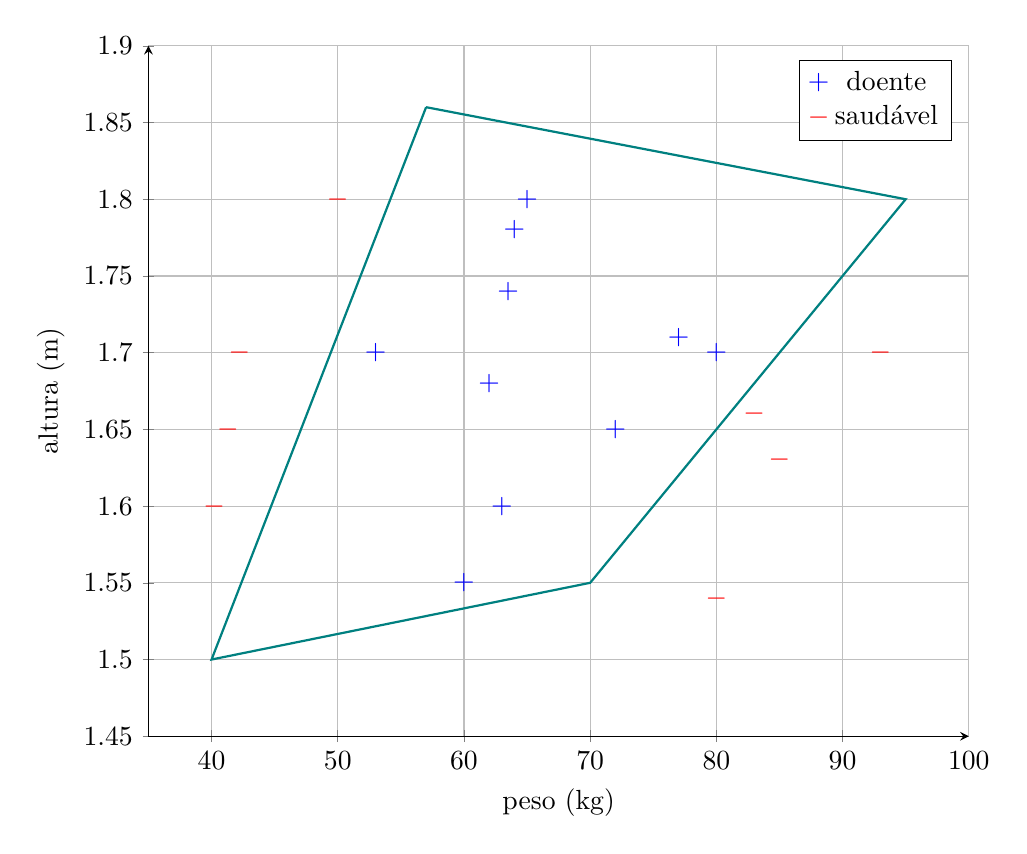
\begin{tikzpicture}
\begin{axis}[axis y line=left, xmin=35, xmax=100, ymin=1.45, ymax=1.9, axis x line=bottom, grid, xlabel=peso (kg),   ylabel=altura (m)]
\addplot[only marks,mark=text,text mark=\C{$+$},mark options={blue,scale=1}] plot coordinates {
    (65,1.8) (53,1.7) (63,1.6) (72,1.65) (60,1.55) (62,1.68) (64,1.78) (63.5,1.74) (80,1.7) (77,1.71)
}; \addlegendentry{doente}
\addplot[only marks,mark=text,text mark=\Q{$-$},mark options={red,scale=1}] plot coordinates {
    (40.2,1.6) (41.3,1.65) (42.2,1.70) (50,1.80) (80,1.54) (83,1.66) (85,1.63) (93,1.7)
}; \addlegendentry{saudável}
\addplot[thick, mark=none, teal] plot coordinates {
    (57,1.86) (40,1.5) (70,1.55) (95,1.8) (57,1.86)
};
\end{axis}
\end{tikzpicture}
\caption{Exemplo de fronteira de decisão.}
\label{fig:fronteiras}
\end{center}
\end{figure}


\textbf{Hipótese} é um conjunto de restrições nos atributos normalmente denominado pela
letra $h$ \citep{mitchell1997machine}.
%definição do livro, eu acho que pode haver outros tipos de hipoteses,
% como por exemplo, restrições num espaço de parâmetros.
Essas restrições delimitam um subconjunto de todos os exemplos possíveis,
pois determinam quais valores cada atributo aceita.
As restrições são as necessárias justamente para que o subconjunto seja somente de exemplos
positivos.
Reunindo-se todas as hipóteses possíveis, tem-se o espaço de hipóteses $H$.
Se houver pelo menos um atributo contínuo (ou discreto com um número infinito de valores),
infinitas hipóteses são possíveis.
Em qualquer caso, evidentemente, podem existir hipóteses diferentes, porém equivalentes.
Assim, pode-se dizer que $H = \{h_i | \forall i \in \mathbb{N}^+\}$.
% (ou seria  $\mathcal{H}$ ??)
Cada $h$ pode ser descrita como uma função do mesmo tipo que $c$, mas que aceita apenas
elementos do conjunto $\mathcal{D} \subseteq X$ de todos os exemplos que efetivamente se
manifestam em uma determinada aplicação:
\begin{equation}
h: \mathcal{D} \rightarrow \{-,+\}
\end{equation}


A tarefa de \textit{aprendizado de conceito}, dado um conjunto de exemplos L CONTIDO EM XxY? $\mathcal{L}:\{\langle \bm{x}_1, c(\bm{x}_1) \rangle, \langle \bm{x}_2, c(\bm{x}_2) \rangle, ... \}$, tem como objetivo encontrar uma hipótese $h \in H,$ tal que
\begin{equation}
 h(\bm{x}) = c(\bm{x}), \forall \bm{x} \in \mathcal{D}
\end{equation}
Porém, como tem-se apenas o conjunto $\mathcal{L}$, é preciso assumir que ele é representativo de $\mathcal{D}$.
Esse é o princípio do aprendizado indutivo: é possível \textbf{predizer} a classe de novos exemplos baseando-se num conjunto de \textbf{treinamento}.
Logo, o resultado da indução é um \textbf{modelo} de representação (DENOMINADO $\theta$) de parte da realidade; capaz de ser usado na generalização de fatos conhecidos para novas situações.

Além de depender de $\mathcal{L}$, a hipótese $h$ depende da \textit{linguagem de representação} e
do \textit{viés de busca}.
Ambas são definidas pelo algoritmo de aprendizado.
O modelo $\theta$ é descrito pela linguagem de representação,
pois ela é a forma de se representar o conhecimento adquirido -
árvores de decisão, neurônios artificiais etc. \citep{quinlan1993c4,haykin1994neural}.
O \textit{viés de busca}, por sua vez, é a forma do processo de construção do modelo dentro da linguagem -
heurística gulosa, otimização de funções etc.
Da mesma forma, os parâmetros do algoritmo também influenciam a elaboração de $h$.
Esses fatores fazem com que o aprendizado de qualquer modelo seja enviesado.

Em muitos casos, para se gerar $\mathcal{L}$, pode-se amostrar para rotulação apenas
parte de um conjunto de exemplos não rotulados $\mathcal{U}$ tendo em vista
restrições de custo.
A ordem de escolha dos exemplos de treinamento, quando não é fortuita ou
intencionalmente aleatória, também é caracterizada por um viés.
Esse viés é característico do aprendizado ativo abordado no
Capítulo \ref{cap:aprendizado-ativo} e é um dos pontos de investigação propostos
no Capítulo \ref{cap:plano} enquanto influência na construção de $h$.


% \e{\textbf{preciso definir} conjunto de validação . . .  classificador}
%
% \e{\textbf{preciso definir} conhecimento . . . }
%
% \e{\textbf{preciso definir} variância. . .   }